%%%%%%%%%%%%%%%%%%%%%%%%%%%%%%%%%%%%%%%%%%%%%%%%%%%
%% Capítulo 2: Iteración
%%%%%%%%%%%%%%%%%%%%%%%%%%%%%%%%%%%%%%%%%%%%%%%%%%%

Como hemos podido comprobar en el capítulo anterior, muchos de los fractales clásicos son generados repitiendo indefinidamente un proceso. Iteración es el proceso de repetir una y otra vez un método, ocasionalmente sobre el resultado de la aplicación anterior. La evolución de este procedimiento es a lo que llamamos un \textbf{sistema dinámico}, y aplicar esta metodología sobre ciertos lugares del plano y sobre ciertas funciones comlejas $f:\C\longrightarrow\C$ es lo que nos proporcionará bellas imágenes fractales.

\section{Iteración en $\R$}
\begin{definicion}
    Consideramos una función $f:\R\longrightarrow\R$ y un punto $x\in\R$. La aplicación sucesiva de $f$ a $x$ -- \textit{i.e.} $x,f(x),f(f(x)), f(f(f(x))),\dots$ -- produce las \textit{iteradas} de la función $f$ en el punto $x$. Al conjunto de dichas iteradas se le denomina \textit{órbita} $O_f(x)$ de $f$ en $x$.
    $$
    O_f(x):=\left\lbrace x, f(x), f^2(x), \dots, f^n(x), \dots\right\rbrace.
    $$
    donde $f^n$ denota a $f\circ f^{n-1}$.
\end{definicion}

Lo siguiente es plantearse la posible convergencia de la sucesión $\{f^n(x)\}$. Para ello, y a partir de este momento nos ayudaremos del software \textcolor{blue}{\href{https://www.wolfram.com/mathematica/}{Mathematica®}} en su versión 12 (concretamente la versión 12.1). El comando \verb|NestList[f,x,n]| itera una función \verb|f|, comenzando en el punto \verb|x| \verb|n| veces y devuelve una lista con los \verb|n| valores. 

\begin{verbatim}
In[]:= NestList[f, a, 5]

Out[]= {a, f[a], f[f[a]], f[f[f[a]]], f[f[f[f[a]]]], 
        f[f[f[f[f[a]]]]]}
\end{verbatim}

Para saber qué ocurre a largo plazo podemos iterar un número grande de veces, fijémonos lo que ocurre si utilizamos $f(x):=\sqrt{x}$ comenzando por $x_0=0.175$.

\begin{verbatim}
In[]:= f[x_] = Sqrt[x];
    NestList[f, 0.175, 20]
    
Out[]= {0.175, 0.41833, 0.646784, 0.804229, 0.896788, 0.946989, 
    0.973134, 0.986475, 0.993215, 0.996602, 0.998299, 0.999149, 
    0.999575, 0.999787, 0.999894, 0.999947, 0.999973, 0.999987, 
    0.999993, 0.999997, 0.999998}
\end{verbatim}

Como se puede observar, en cada iteración se acerca cada vez más a $1$, lo cual denotamos con $O_f(0.175)\rightarrow 1$. Nuestro objetivo ahora es poder conocer el comportamiento de la órbita de una función y un punto dados. 

\subsection{Tipos de convergencia}

Para ilustrar de forma sencilla las distintas posibilidades nos ayudaremos de la función $f:\R\longrightarrow\R^+$ definida como $f(x)=x^2$. Es claro que si $|x|>1$ entonces $O_f(x)\rightarrow\infty$, es decir, diverge. Si $|x|<1$ se tiene que $O_f(x)\rightarrow 0$, por lo tanto converge a $0$. Por último, en caso de que $x=-1$ ó $x=1$ tenemos $O_f(x)=\{1\}$ en ambos casos, por lo que lógicamente convergen a $1$.

En este caso, y debido a la simplicidad de la función, hemos podido clasificar la órbita de todos los puntos de $\R$, pudiendo decir que todas las órbitas son \textit{predecibles}. Pensemos ahora en la función $g:\R\longrightarrow\R$ definida como $g(x)=-x^3$. De nuevo, si $|x|<1$ la órbita converge a 0 y si $|x|>1$ la órbita diverge, aunque este caso lo hagan cambiando ocasionalmente el signo. Sin embargo, en $x=-1$ y en $x=1$ ocurre un suceso distinto.
$$
O_g(1) = \{-1,1,-1,1,\dots\}
$$
$$
O_g(-1) = \{1,-1,1,-1,\dots\}
$$
Los valores $1$ y $-1$ se van alternando. Esto es, la órbita no es convergente, ni divergente, sino cíclica, concretamente de período 2. A este caso se le denomina \textbf{órbita periódica}. Aunque este caso sea distinto, aún es predecible, podemos saber cómo se comportará la órbita en el infinito. Pero veamos ahora un último ejemplo distinto, con la función $h:\R\longrightarrow\R$ definida como $h(x)=4x(1-x)$ en el punto $x=0.3$:

\begin{verbatim}
In[]:= h[x_] = 4 x (1 - x);
    NestList[h, 0.3, 20]

Out[]= {0.3, 0.84, 0.5376, 0.994345, 0.0224922, 0.0879454, 
    0.320844, 0.871612, 0.447617, 0.989024, 0.0434219, 
    0.166146, 0.554165, 0.988265, 0.0463905, 0.176954, 
    0.582565, 0.972732, 0.106097, 0.379361, 0.941785}
\end{verbatim}

Esta vez la órbita no sigue ningún patrón predecible, y además se puede comprobar que es muy sensible a las condiciones iniciales. A esto le llamamos un comportamiento \textbf{caótico}.

\subsection{Velocidad de convergencia}

En estos casos, han sido suficientes 20 iteraciones para conocer el comportamiento de la órbita a largo plazo, pero interesa saber cuántas iteraciones son necesarias en cada punto para saber si hemos alcanzado el valor al que converge la sucesión. En general, este alcance se toma como aproximado, pues generalmente nunca se llega a alcanzar el punto fijo, tan solo podemos reducir la diferencia tanto como queramos. En este sentido, \textit{Mathematica} tiene dos comandos útiles:

\begin{itemize}
    \item \verb|FixedPointList[f,expr]| genera una lista de valores resultantes de aplicar \verb|f| a \verb|expr| repetidamente hasta que los dos últimos valores no cambian. Para parametrizar la precisión en la proximidad de los valores podemos utilizar el argumento opcional \verb|SameTest|\footnote{Más información en la documentación oficial \url{https://reference.wolfram.com/language/ref/FixedPointList.html}}.
    \item \verb|FixedPoint[f,expr]| hace lo mismo pero produce como salida únicamente el valor último producido.
\end{itemize}

El siguiente código muestra un ejemplo de uso:

\begin{verbatim}
In[]:= f[x_] = x/2 + 1/x;
    FixedPointList[f, 1.0, SameTest -> (Abs[#1 - #2] < 10^-4 &)]
    FixedPoint[f, 1.0]

Out[]= {1., 1.5, 1.41667, 1.41422, 1.41421}
Out[]= 1.41421
\end{verbatim}

Y a partir de la longitud de la lista que nos devuelve \verb|FixedPointList|, es decir, con el sencillo comando \verb|Length[FixedPoint[f,x]]| podemos medir la velocidad de convergencia de cada punto.

\section{Iteración en $\C$}

De manera natural, todos los conceptos explicados anteriormente sobre iteración en $\R$ se pueden extender al plano complejo. Esto es, dada una función compleja $f:\C\longrightarrow\C$ y un número complejo $z\in\C$, podemos preguntarnos por el comportamiento a largo plazo de la órbita $O_f(z)$. En este caso, y utilizando la correspondencia entre un punto $(x,y)\in\R^2$ y un número complejo $z=x+i\cdot y$, podemos representar cada punto de una órbita como un punto del plano, pudiendo así fácilmente graficar las órbitas y observar su comportamiento. Observamos en la imagen \ref{fig:orbitas-C} dos ejemplos de esto, ambos han sido generados por el código siguiente, cambiando necesariamente los parámetros para generar la figura (b), de aspecto más armónico.

\begin{verbatim}
In[]:= f[z_] := z^2;
    x0 = 0.9 + 0.3 I;
    ComplexListPlot[N[FixedPointList[f, x0, 10]]];
    ComplexListPlot[N[FixedPointList[f, x0, 10]], Joined -> True];
    Show[%, %%]
\end{verbatim}

\begin{figure}[h]
    \begin{tabular}{cc}
      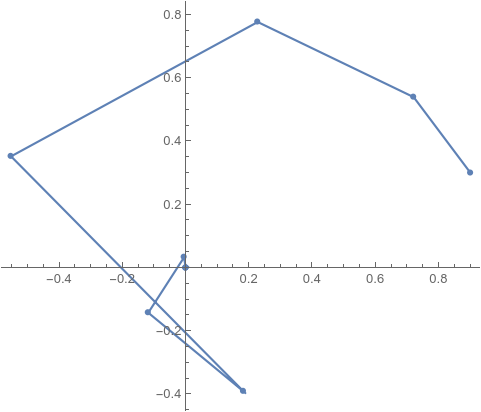
\includegraphics[scale=0.45]{./img/orbita-1.png} &   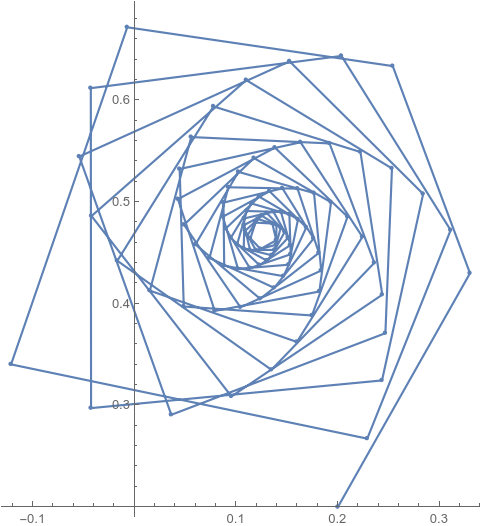
\includegraphics[scale=0.4]{./img/orbita-2.png} \\
    (a)$f(z)=z^2$ en $z=0.9+0.3i$ & (b) $f(z)=z^2+0.33+0.35$ en $z=0.2+0.2i$ \\[6pt]
    \end{tabular}
    \caption{Representación de dos órbitas en $\C$}
    \label{fig:orbitas-C}
\end{figure}

De hecho, para la función $f(z)=z^2$ se tiene que la órbita de todo $z$ con módulo $|z|<1$ tiende a $0$, mientras que si $|z|>1$ diverge y si $|z|=1$ su órbita permanece siempre en la esfera unidad $S^1$. Por tanto, $S^1$ se convierte en la frontera entre los puntos \textit{de escape} -- cuyas órbitas escapan -- y los puntos \textit{prisioneros} -- cuyas órbiras convergen. Por tanto los puntos del plano complejo presentan una dicotomía para la función $f$: escapar o no. $S^1$, al ser la frontera entre estos dos conjuntos, es conocido como el \textit{conjunto de Julia} de la función $f(z)=z^2$. Esta idea será tratada detenidamente en el capítulo \ref{chap:Julia-Mandelbrot}.

\section{El método de Newton y cuencas de atracción}

La iteración es la base de muchos métodos numéricos, entre los que en este caso destacamos el `método de Newton', el cual fue inicialmente descrito por \textit{Isaac Newton} en su libro \textit{De analysi per aequationes numero terminorum infinitas}. Este es un procedimiento muy útil y utilizado en la resolución de ecuaciones, tomando una ecuación como el punto en el que se anula una función $f:\R\longrightarrow\R$, aunque gracias al trabajo de \textit{Arthur Cayley} sabemos que es posible generalizarlo a los números complejos.

Recordemos que dada una ecuación $f(z)=0$ para cierta función compleja y derivable $f:\C\longrightarrow\C$, el método de Newton itera la función
\begin{equation}
    \label{eq:metodo-Newton}
    N_f(z)=z-\frac{f(z)}{f'(z)}
\end{equation} 
comenzando por un punto $z_0$ cercano a la raíz. Es decir, calcula la sucesión $\{z_n\}$ definida como $z_{n+1}=N_f(z_n) \ \forall n\in\N$, la cual converge a un punto $a\in\C$ que verifica $f(a)=0$.

Sin embargo, en muchas ecuaciones, comenzando por las polinómicas de grado mayor que 1, existen varias soluciones distintas, pero el método de Newton converge sólo a una de ellas. Nuestro objetivo ahora se sitúa en discernir, para cada punto $z_0$ del plano, a qué solución de la ecuación $f(z)=0$ converge la sucesión $\{z_n\}$ dada por el método de Newton utilizando a $z_0$ como semilla. En las siguientes secciones veremos algunos ejemplos de esta distinción y su utilidad, llegando a las primeras imágenes fractales generadas por iteración.

\subsection{Caso $z^2-1$}

Consideramos la función compleja $f:\C\longrightarrow\C$ dada por $f(z)=z^2-1$, la cual tiene dos raíces: $1$ y $-1$, las dos raíces cuadradas de 1. Una forma sencilla de comprobar a qué raíz converge cada sucesión utilizando como semilla cada $z_0\in\C$ es asociando un color a cada punto del plano dependiendo de la raíz a la que converja y pidiendo a \textit{Mathematica} que coloree el plano complejo siguiendo este criterio:

\begin{verbatim}
In[]:= iteracionN = #2 - #1[#2]/Derivative[1][#1][#2] &;
    newtonArgumento = 
      Compile[{{z, _Complex}}, 
       Arg[FixedPoint[iteracionNR[f, #] &, z, 50]]];
    
In[]:= DensityPlot[newtonArgumento[x + I*y], {x, -2, 2}, {y, -2, 2}, 
     PlotPoints -> 100, Mesh -> False, ColorFunction -> "Rainbow"] 
\end{verbatim}

\begin{figure} [h]
\centering
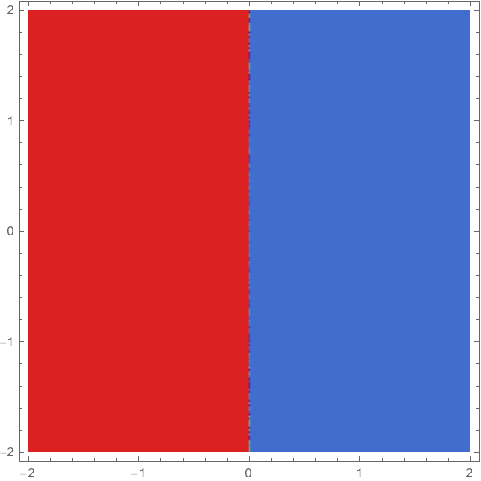
\includegraphics[scale = 0.4]{img/cuencas-1.png}
\caption{Cuencas de atracción de $f(z)=z^2-1$.}
    \label{fig:cuencas-1}
\end{figure}

Produciendo como resultado la imagen \ref{fig:cuencas-1}. Como podemos ver, y teniendo en cuenta que la imagen solo grafica el intervalo $[-2,2]\times[-2,2]$ y un número finito de puntos\footnote{El número de puntos que se grafica se puede parametrizar con el argumento opcional PlotPoints| de las funciones |Plot|. A mayor valor mayor calidad de imagen y resolución, pero mayor tiempo de ejecución.} la sucesión cuya semilla es un punto perteneciente al semiplano abierto de la derecha converge a la raíz $1$. Por otro lado, si la sucesión comienza con un complejo del semiplano abierto de la izquierda, entonces esta converge a la raíz $-1$. Apoyándonos en este ejemplo, definimos el siguiente concepto.

\begin{definicion}[Cuenca de atracción]
    Definimos como \textit{cuenca de atracción} de una raíz $a\in\C$ de una función compleja $f:\C\longrightarrow\C$ (\textit{i.e.} $f(a)=0$), y denotamos como $A(a)$ al conjunto de puntos $z_0\in\C$ tales que la sucesión $\{z_n\}$ dada por $z_{n+1}=N_f(z_n)$ converge a $a$ utilizando a $z_0$ como primer valor de la sucesión. 
\end{definicion}

Es decir, tenemos en este caso que
$$
A(-1)=\{z\in\C:\operatorname{Re}z<0\},
$$
$$
A(1)=\{z\in\C:\operatorname{Re} z>0\}
$$
y sin embargo los puntos del eje $Y$ no convergen a ninguna de las raíces, siendo esta por tanto la frontera entre las dos cuencas de atracción. 


